\section{Results}
\label{sec:results}

% I write the description of the plots in their caption. In a succesive step of the work we can move the plot descriptions in the text.

\begin{table}[h!]
	\caption{Error before processing HMM}
	\centering
	\begin{tabular}{|c |c c c|}
	\hline
	$r_{test}$ & CENS & CLP & CRP\\ \hline
	0.1 & 0.4946 & 0.4739 & 0.6206\\
	0.2 & 0.4657 & 0.6000 & 0.6376\\
	0.3 & 0.4765 & 0.5691 & 0.5803\\
	\hline
	\end{tabular}
\end{table}

\begin{table}[h!]
	\caption{Error after processing HMM}
	\centering
	\begin{tabular}{|c |c c c|}
	\hline
	$r_{test}$ & CENS & CLP & CRP\\ \hline
	0.1 & 0.4439 & 0.4502 & 0.5641\\
	0.2 & 0.4296 & 0.5919 & 0.5967\\
	0.3 & 0.4179 & 0.5484 & 0.5204\\
	\hline
	\end{tabular}
\end{table}

\begin{figure} [h!]
	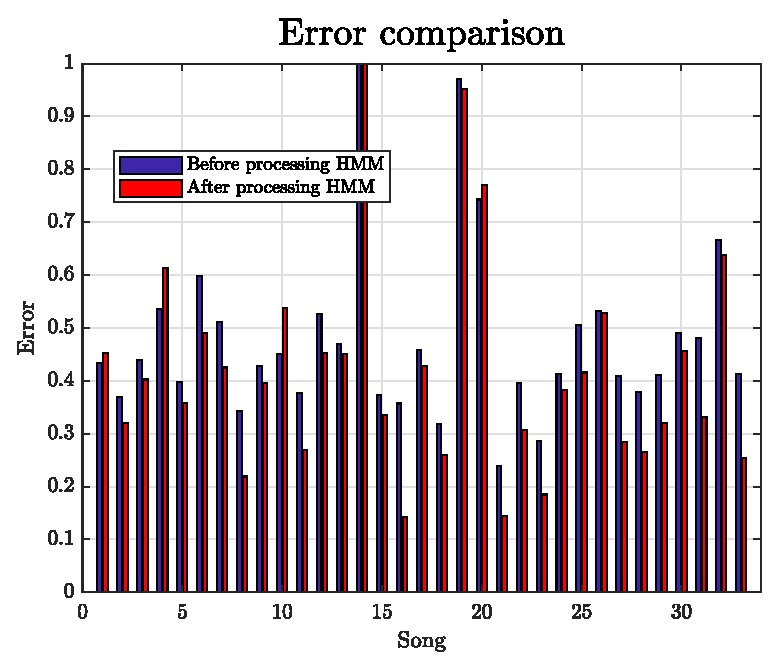
\includegraphics[width=0.5\textwidth]{img/Result_HMM/CENS/plot03071}
	\caption{Error comparison using CENS features (train = 0.7; test = 0.3). It is the one that has given the best results. We notice that a lot of songs have been discarded by Viterbi and therefore we have only 33 songs (not 150*0.3=45 as expected)}
\end{figure}

\begin{figure} [h!]
	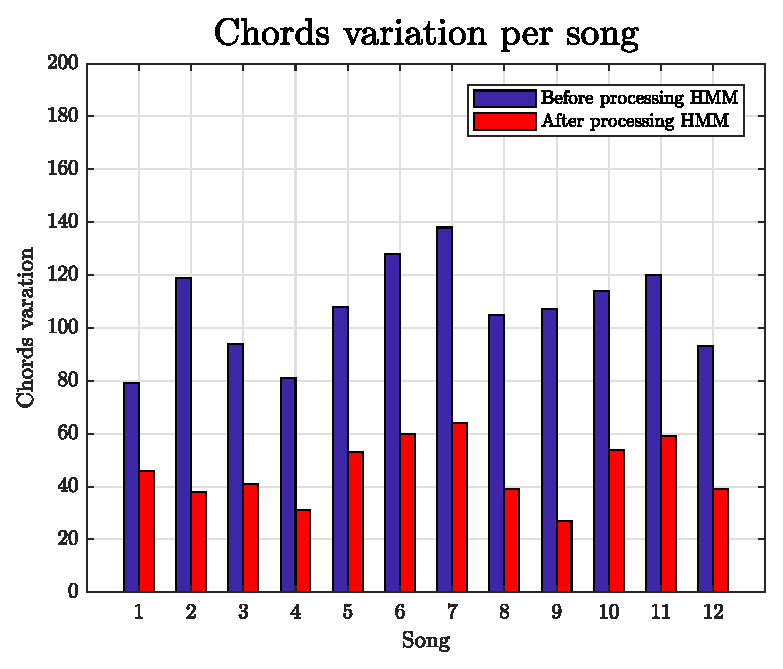
\includegraphics[width=0.5\textwidth]{img/Result_HMM/SMOOTHING/SmoothPerSongCENS0109}
	\caption{Chords variation per song using CENS features (train = 0.9; test = 0.1)}
\end{figure}

\begin{figure} [h!]
	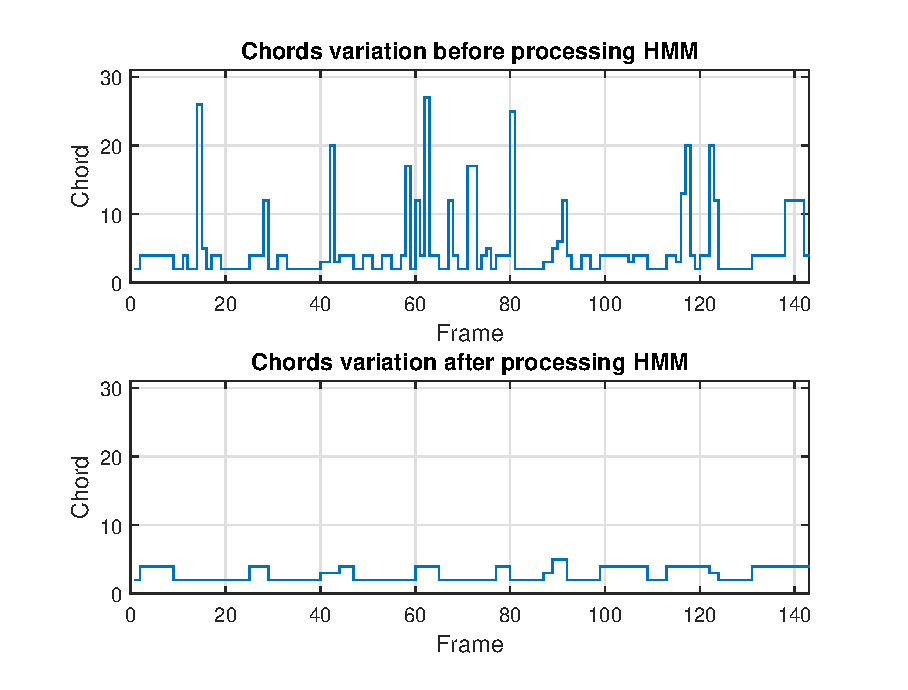
\includegraphics[width=0.5\textwidth]{img/Result_HMM/SMOOTHING/SmoothSingleSongCENS0109}
	\caption{Chord variation in a single song using CENS features (train = 0.9; test = 0.1); it represents the second song of the plot of the smoothing of all song}
\end{figure}
